% !TeX spellcheck=en_US

% This is the ACL 2018 template as the 2019 template is not available yet
% TODO: update to the 2019 template

\documentclass[11pt,a4paper]{article}
\usepackage[hyperref]{acl2018}
\usepackage{times}
\usepackage{latexsym}

\usepackage{url}

% Packages and definitions added by Max

% Acronyms
\usepackage[single, list-caps=true]{acro}
% !TeX root=main.tex
% !TeX spellcheck=en_US

\DeclareAcronym{hipaa}{
    short = HIPAA,
    long = Health Insurance Portability Accountability Act,
    extra = {American health care law.},
}
\DeclareAcronym{phi}{
    short = PHI,
    long = protected health information,
}
\DeclareAcronym{ehr}{
    short = EHR,
    long = electronic health record,
}
\DeclareAcronym{nlp}{
    short = NLP,
    long = natural language processing,
    short-indefinite = an,
}
\DeclareAcronym{ner}{
    short = NER,
    long = named entity recognition,
    short-indefinite = an,
}
\DeclareAcronym{crf}{
    short = CRF,
    long = conditional random field,
}
\DeclareAcronym{mlp}{
    short = MLP,
    long = multi-layer perceptron,
    short-indefinite = an,
}
\DeclareAcronym{rnn}{
    short = RNN,
    long = recurrent neural network,
    short-indefinite = an,
}
\DeclareAcronym{lstm}{
    short = LSTM,
    long = long short-term memory,
    short-indefinite = an,
}
\DeclareAcronym{elmo}{
    short = ELMo,
    long = embeddings from language models,
}
\DeclareAcronym{dann}{
    short = DANN,
    long = domain-adversarial neural network,
}


% Math
\usepackage{amsmath}
\usepackage{bm}
\usepackage{mathtools}
\DeclarePairedDelimiter{\abs}{\lvert}{\rvert}
\DeclarePairedDelimiter{\norm}{\lVert}{\rVert}
\usepackage{xspace}
\newcommand{\fone}{\ensuremath{F_1}\xspace}
\newcommand{\ltwo}{\ensuremath{L^2}\xspace}

% Bib (mostly for autocompletion)
\usepackage{natbib}

% References
\usepackage[capitalise]{cleveref}

% TikZ
\usepackage{tikz}
\usetikzlibrary{arrows, backgrounds, calc, scopes, fit, intersections, matrix, positioning, shapes, shapes.misc}

% Frames
\usepackage{framed}

% Strikethrough
\usepackage[normalem]{ulem}
% Tables
\usepackage{booktabs}

%\aclfinalcopy % Uncomment this line for the final submission
%\def\aclpaperid{***} %  Enter the acl Paper ID here

%\setlength\titlebox{5cm}
% You can expand the titlebox if you need extra space
% to show all the authors. Please do not make the titlebox
% smaller than 5cm (the original size); we will check this
% in the camera-ready version and ask you to change it back.

\title{Adversarial Learning of Text Representations for De-Identification of Medical Records}

\author{First Author \\
    Affiliation / Address line 1 \\
    Affiliation / Address line 2 \\
    Affiliation / Address line 3 \\
    {\tt email@domain} \\\And
    Second Author \\
    Affiliation / Address line 1 \\
    Affiliation / Address line 2 \\
    Affiliation / Address line 3 \\
    {\tt email@domain} \\}

\date{}

\begin{document}
\maketitle

% !TeX root=main
% !TeX spellcheck=en_US

\begin{abstract}
    TODO
\end{abstract}

% !TeX root=main
% !TeX spellcheck=en_US

\section{Introduction}\label{sec:introduction}
%
In addition to structured medical data, electronic health records contain free-text patient notes that are a rich source of information.
%
Due to privacy and data protection laws, medical records can only be shared and used for research if they are sanitized.
%
De-identification is the task of finding and labeling \ac{phi} in medical text for sanitization.
%
\Ac{phi} includes potentially identifying information such as names, professions, geographic identifiers, dates, and account numbers.
%
The American \ac{hipaa} defines 18 categories of \ac{phi}.

% TODO Why is it important (enable large-scale studies)

%
Trying to train a software tool for automatic de-identification leads to a ``chicken and egg problem''~\citep{uzuner2007evaluating}: without a comprehensive training set, an automatic de-identification tool cannot be developed, but without such a tool, it is difficult to share de-identified medical text for research (including for training the tool itself).
%
The standard method of data protection compliant sharing of training data for a de-identification tool requires humans to pseudonymize protected information with substitutes (replacing e.g.\ every person name with a different person name and every date with a different date) in a document-coherent way \cite{uzuner2007evaluating}.

% TODO including applying spelling mistakes to the substitutes etc

% Why is manual pseudonymization not so great? (time-consuming, coherency)
%
Today, a pseudonymized dataset for de-identification from a single source is publicly available \citep{stubbs2015annotating}.
%
However, de-identification tools trained on the dataset are too specific for the concrete data and do not generalize well to data from other sources~\citep{stubbs2017identification}.
%
If a medical institution instead decides to train a de-identification tool on their raw text data, it is conceivable that the tool would contain traces of the \ac{phi} it was trained with, making it possible for an attacker to recover parts of the training data if the tool itself is shared.
%
To achieve a universal de-identification tool, many medical institutions would have to pool their data.
%
Preparing this data for sharing using the document-coherent pseudonymization approach requires large human effort \citep{dernoncourt2017identification}.

% Why is sharing training data the best solution for a de-identification model?
%
We introduce two representation approaches to privacy-preserving sharing of medical text that allow training a de-identification tool: an automatic pseudonymization and an adversarially learned private representation.
%
Our approaches still requires humans to annotate \ac{phi} (as this is the training data for the task) but the pseudonymization step is performed by the transformation to the representations.
%
A tool trained on our representations could easily be made publicly available because its parameters cannot contain any protected data, as it is never trained on raw text.
%
Simplifying the de-identification procedure may enable large-scale medical studies that are otherwise too costly.

% TODO present results
% use acronym short forms here (\acs{…}) and explain them later
We train a basic \acs{lstm}-\acs{crf} de-identification model on raw and automatically pseudonymized text as well as on our adversarial private representation.
%


% !TeX root=main
% !TeX spellcheck=en_US

\section{Related Work}\label{sec:related}
%


\subsection{Automatic De-Identification}
In 2006, 2014 and 2016, three shared tasks on de-identification were organized by the i2b2 group.
%
The organizers performed manual pseudonymization on clinical records from a single source to create the datasets for each of the shared tasks \citep{stubbs2015annotating}.
%
An \fone score of $95\%$ has been suggested as a target for reasonable de-identification systems \citep{stubbs2015automated}.

%
Up to the 2014 shared task, the organizers emphasized that it is unclear if a tool trained on the provided datasets will generalize to medical records from other sources \citep{uzuner2007evaluating,stubbs2015automated}.
%
The 2016 shared task featured a sight-unseen track in which existing systems were evaluated on records from a new data source.
%
The best system achieved an \fone score of only $79\%$, proving that de-identification systems at the time were not able to deliver sufficient performance on completely new data \citep{stubbs2017identification}.

%
\citet{dernoncourt2017identification} achieve state-of-the-art performance in de-identification with \iac{lstm} model.
%
Their model achieves an \fone score of $97.85\%$ on the i2b2 2014 dataset.
%
Using transfer learning from a model trained on a larger dataset, they were able to further improve their scores on the i2b2 2014 dataset \citep{lee2017transfer}.
%
It is possible to reach an $98\%$ \fone score on the i2b2 2014 dataset by using document position information as an additional input \citep{zhao2018leveraging}, which will, however, most likely deteriorate generalization performance to instances of medical text with different structures.

\subsection{Adversarial Representation Learning}
%
Adversarial learning for deep learning models was popularized by \citet{goodfellow2014generative}.
%

The \ac{dann} architecture \citep{ganin2016domain} implements a three-party game 

\begin{itemize}
    \item Learning fair representations \citep{zemel2013learning}
    \item \Ac{dann} architecture \citep{ganin2016domain}
    \item Uses in anonymization / demographics independent representation \citet{elazar2018adversarial,li2018towards}
    \item \citet{elazar2018adversarial} cautionary conclusion (continued adversary training beats the representation)
    \item \citet{feutry2018learning} three-step learning procedure
\end{itemize}

% !TeX root=main
% !TeX spellcheck=en_US

\section{De-Identification Model}\label{sec:deidentification-model}
%
Our de-identification model uses a bidirectional \ac{lstm}-\ac{crf} architecture that has been proven to work well in sequence tagging \citep{huang2015bidirectional,lample2016neural} and de-identification \citep{dernoncourt2017identification,liu2017identification}.
%
In addition to pre-trained FastText \citep{bojanowski2016enriching} or GloVe \citep{pennington2014glove} word embeddings, it uses the casing feature from \citet{reimers2017optimal} as an input.
%
The feature maps words to a one-hot representation of their casing (\textit{numeric}, \textit{mainly numeric}, \textit{all lower}, \textit{all upper}, \textit{initial upper}, \textit{contains digit}, or \textit{other}).

%
When trained on the raw i2b2 2014 data, our models achieve comparable \fone scores to the state of the art (see \cref{tab:baseline-results}).
%
The casing feature improves GloVe by $0.4$ percentage points.

\begin{table}
    \centering
    \begin{tabular}{ll}
        \toprule
        Model & \fone (\%)\\
        \midrule
        % python -m deid.tools.graphics.baseline_table
        % \Ac{elmo} & $97.74$ \\
        Our FastText & $97.67$ \\
        Our GloVe & $97.62$ \\
        \citet{dernoncourt2017identification} & $\bm{97.85}$\\
    \end{tabular}
    \caption{Average precision, recall, and \fone scores of our de-identification models in comparison to the state of the art.}\label{tab:baseline-results}
\end{table}
% !TeX root=main
% !TeX spellcheck=en_US

\section{Automatic Pseudonymization}\label{sec:automatic-pseudonymization}
%
As state-of-the-art de-identification models do not rely on document coherency to identify \ac{phi}, we evaluate a naive word-level automatic pseudonymization approach to perturbing training data.
%
Before training, we replace all \ac{phi} tokens with a random choice of a fixed number $N$ of their neighbors in an embedding space, as determined by cosine distance in a pre-computed embedding matrix.

%
When using GloVe embeddings, only tokens that exist in the pre-computed embedding matrix are moved to their neighbors.
%
The unknown token is not modified as it does not contain any information (except that the token in question is not part of the precomputed matrix).

\begin{figure}
    \centering
    %% Creator: Matplotlib, PGF backend
%%
%% To include the figure in your LaTeX document, write
%%   \input{<filename>.pgf}
%%
%% Make sure the required packages are loaded in your preamble
%%   \usepackage{pgf}
%%
%% Figures using additional raster images can only be included by \input if
%% they are in the same directory as the main LaTeX file. For loading figures
%% from other directories you can use the `import` package
%%   \usepackage{import}
%% and then include the figures with
%%   \import{<path to file>}{<filename>.pgf}
%%
%% Matplotlib used the following preamble
%%   \usepackage{fontspec}
%%   \setmainfont{Times New Roman}
%%   \setsansfont{Lucida Grande}
%%   \setmonofont{Andale Mono}
%%
\begingroup%
\makeatletter%
\begin{pgfpicture}%
\pgfpathrectangle{\pgfpointorigin}{\pgfqpoint{3.000000in}{2.500000in}}%
\pgfusepath{use as bounding box, clip}%
\begin{pgfscope}%
\pgfsetbuttcap%
\pgfsetmiterjoin%
\definecolor{currentfill}{rgb}{1.000000,1.000000,1.000000}%
\pgfsetfillcolor{currentfill}%
\pgfsetlinewidth{0.000000pt}%
\definecolor{currentstroke}{rgb}{1.000000,1.000000,1.000000}%
\pgfsetstrokecolor{currentstroke}%
\pgfsetdash{}{0pt}%
\pgfpathmoveto{\pgfqpoint{0.000000in}{0.000000in}}%
\pgfpathlineto{\pgfqpoint{3.000000in}{0.000000in}}%
\pgfpathlineto{\pgfqpoint{3.000000in}{2.500000in}}%
\pgfpathlineto{\pgfqpoint{0.000000in}{2.500000in}}%
\pgfpathclose%
\pgfusepath{fill}%
\end{pgfscope}%
\begin{pgfscope}%
\pgfsetbuttcap%
\pgfsetmiterjoin%
\definecolor{currentfill}{rgb}{1.000000,1.000000,1.000000}%
\pgfsetfillcolor{currentfill}%
\pgfsetlinewidth{0.000000pt}%
\definecolor{currentstroke}{rgb}{0.000000,0.000000,0.000000}%
\pgfsetstrokecolor{currentstroke}%
\pgfsetstrokeopacity{0.000000}%
\pgfsetdash{}{0pt}%
\pgfpathmoveto{\pgfqpoint{0.620278in}{0.550778in}}%
\pgfpathlineto{\pgfqpoint{2.808850in}{0.550778in}}%
\pgfpathlineto{\pgfqpoint{2.808850in}{2.186667in}}%
\pgfpathlineto{\pgfqpoint{0.620278in}{2.186667in}}%
\pgfpathclose%
\pgfusepath{fill}%
\end{pgfscope}%
\begin{pgfscope}%
\pgfpathrectangle{\pgfqpoint{0.620278in}{0.550778in}}{\pgfqpoint{2.188572in}{1.635889in}}%
\pgfusepath{clip}%
\pgfsetbuttcap%
\pgfsetmiterjoin%
\definecolor{currentfill}{rgb}{0.498039,0.498039,0.498039}%
\pgfsetfillcolor{currentfill}%
\pgfsetfillopacity{0.100000}%
\pgfsetlinewidth{1.003750pt}%
\definecolor{currentstroke}{rgb}{0.498039,0.498039,0.498039}%
\pgfsetstrokecolor{currentstroke}%
\pgfsetstrokeopacity{0.100000}%
\pgfsetdash{}{0pt}%
\pgfpathmoveto{\pgfqpoint{0.620278in}{1.471993in}}%
\pgfpathlineto{\pgfqpoint{2.808850in}{1.471993in}}%
\pgfpathlineto{\pgfqpoint{2.808850in}{2.186667in}}%
\pgfpathlineto{\pgfqpoint{0.620278in}{2.186667in}}%
\pgfpathclose%
\pgfusepath{stroke,fill}%
\end{pgfscope}%
\begin{pgfscope}%
\pgfsetbuttcap%
\pgfsetroundjoin%
\definecolor{currentfill}{rgb}{0.000000,0.000000,0.000000}%
\pgfsetfillcolor{currentfill}%
\pgfsetlinewidth{0.803000pt}%
\definecolor{currentstroke}{rgb}{0.000000,0.000000,0.000000}%
\pgfsetstrokecolor{currentstroke}%
\pgfsetdash{}{0pt}%
\pgfsys@defobject{currentmarker}{\pgfqpoint{0.000000in}{-0.048611in}}{\pgfqpoint{0.000000in}{0.000000in}}{%
\pgfpathmoveto{\pgfqpoint{0.000000in}{0.000000in}}%
\pgfpathlineto{\pgfqpoint{0.000000in}{-0.048611in}}%
\pgfusepath{stroke,fill}%
}%
\begin{pgfscope}%
\pgfsys@transformshift{0.642725in}{0.550778in}%
\pgfsys@useobject{currentmarker}{}%
\end{pgfscope}%
\end{pgfscope}%
\begin{pgfscope}%
\pgftext[x=0.642725in,y=0.453556in,,top]{\sffamily\fontsize{8.000000}{9.600000}\selectfont \(\displaystyle {10^{0}}\)}%
\end{pgfscope}%
\begin{pgfscope}%
\pgfsetbuttcap%
\pgfsetroundjoin%
\definecolor{currentfill}{rgb}{0.000000,0.000000,0.000000}%
\pgfsetfillcolor{currentfill}%
\pgfsetlinewidth{0.803000pt}%
\definecolor{currentstroke}{rgb}{0.000000,0.000000,0.000000}%
\pgfsetstrokecolor{currentstroke}%
\pgfsetdash{}{0pt}%
\pgfsys@defobject{currentmarker}{\pgfqpoint{0.000000in}{-0.048611in}}{\pgfqpoint{0.000000in}{0.000000in}}{%
\pgfpathmoveto{\pgfqpoint{0.000000in}{0.000000in}}%
\pgfpathlineto{\pgfqpoint{0.000000in}{-0.048611in}}%
\pgfusepath{stroke,fill}%
}%
\begin{pgfscope}%
\pgfsys@transformshift{1.140541in}{0.550778in}%
\pgfsys@useobject{currentmarker}{}%
\end{pgfscope}%
\end{pgfscope}%
\begin{pgfscope}%
\pgfsetbuttcap%
\pgfsetroundjoin%
\definecolor{currentfill}{rgb}{0.000000,0.000000,0.000000}%
\pgfsetfillcolor{currentfill}%
\pgfsetlinewidth{0.803000pt}%
\definecolor{currentstroke}{rgb}{0.000000,0.000000,0.000000}%
\pgfsetstrokecolor{currentstroke}%
\pgfsetdash{}{0pt}%
\pgfsys@defobject{currentmarker}{\pgfqpoint{0.000000in}{-0.048611in}}{\pgfqpoint{0.000000in}{0.000000in}}{%
\pgfpathmoveto{\pgfqpoint{0.000000in}{0.000000in}}%
\pgfpathlineto{\pgfqpoint{0.000000in}{-0.048611in}}%
\pgfusepath{stroke,fill}%
}%
\begin{pgfscope}%
\pgfsys@transformshift{1.354939in}{0.550778in}%
\pgfsys@useobject{currentmarker}{}%
\end{pgfscope}%
\end{pgfscope}%
\begin{pgfscope}%
\pgftext[x=1.354939in,y=0.453556in,,top]{\sffamily\fontsize{8.000000}{9.600000}\selectfont \(\displaystyle {10^{1}}\)}%
\end{pgfscope}%
\begin{pgfscope}%
\pgfsetbuttcap%
\pgfsetroundjoin%
\definecolor{currentfill}{rgb}{0.000000,0.000000,0.000000}%
\pgfsetfillcolor{currentfill}%
\pgfsetlinewidth{0.803000pt}%
\definecolor{currentstroke}{rgb}{0.000000,0.000000,0.000000}%
\pgfsetstrokecolor{currentstroke}%
\pgfsetdash{}{0pt}%
\pgfsys@defobject{currentmarker}{\pgfqpoint{0.000000in}{-0.048611in}}{\pgfqpoint{0.000000in}{0.000000in}}{%
\pgfpathmoveto{\pgfqpoint{0.000000in}{0.000000in}}%
\pgfpathlineto{\pgfqpoint{0.000000in}{-0.048611in}}%
\pgfusepath{stroke,fill}%
}%
\begin{pgfscope}%
\pgfsys@transformshift{1.569337in}{0.550778in}%
\pgfsys@useobject{currentmarker}{}%
\end{pgfscope}%
\end{pgfscope}%
\begin{pgfscope}%
\pgfsetbuttcap%
\pgfsetroundjoin%
\definecolor{currentfill}{rgb}{0.000000,0.000000,0.000000}%
\pgfsetfillcolor{currentfill}%
\pgfsetlinewidth{0.803000pt}%
\definecolor{currentstroke}{rgb}{0.000000,0.000000,0.000000}%
\pgfsetstrokecolor{currentstroke}%
\pgfsetdash{}{0pt}%
\pgfsys@defobject{currentmarker}{\pgfqpoint{0.000000in}{-0.048611in}}{\pgfqpoint{0.000000in}{0.000000in}}{%
\pgfpathmoveto{\pgfqpoint{0.000000in}{0.000000in}}%
\pgfpathlineto{\pgfqpoint{0.000000in}{-0.048611in}}%
\pgfusepath{stroke,fill}%
}%
\begin{pgfscope}%
\pgfsys@transformshift{1.852756in}{0.550778in}%
\pgfsys@useobject{currentmarker}{}%
\end{pgfscope}%
\end{pgfscope}%
\begin{pgfscope}%
\pgfsetbuttcap%
\pgfsetroundjoin%
\definecolor{currentfill}{rgb}{0.000000,0.000000,0.000000}%
\pgfsetfillcolor{currentfill}%
\pgfsetlinewidth{0.803000pt}%
\definecolor{currentstroke}{rgb}{0.000000,0.000000,0.000000}%
\pgfsetstrokecolor{currentstroke}%
\pgfsetdash{}{0pt}%
\pgfsys@defobject{currentmarker}{\pgfqpoint{0.000000in}{-0.048611in}}{\pgfqpoint{0.000000in}{0.000000in}}{%
\pgfpathmoveto{\pgfqpoint{0.000000in}{0.000000in}}%
\pgfpathlineto{\pgfqpoint{0.000000in}{-0.048611in}}%
\pgfusepath{stroke,fill}%
}%
\begin{pgfscope}%
\pgfsys@transformshift{2.067154in}{0.550778in}%
\pgfsys@useobject{currentmarker}{}%
\end{pgfscope}%
\end{pgfscope}%
\begin{pgfscope}%
\pgftext[x=2.067154in,y=0.453556in,,top]{\sffamily\fontsize{8.000000}{9.600000}\selectfont \(\displaystyle {10^{2}}\)}%
\end{pgfscope}%
\begin{pgfscope}%
\pgfsetbuttcap%
\pgfsetroundjoin%
\definecolor{currentfill}{rgb}{0.000000,0.000000,0.000000}%
\pgfsetfillcolor{currentfill}%
\pgfsetlinewidth{0.803000pt}%
\definecolor{currentstroke}{rgb}{0.000000,0.000000,0.000000}%
\pgfsetstrokecolor{currentstroke}%
\pgfsetdash{}{0pt}%
\pgfsys@defobject{currentmarker}{\pgfqpoint{0.000000in}{-0.048611in}}{\pgfqpoint{0.000000in}{0.000000in}}{%
\pgfpathmoveto{\pgfqpoint{0.000000in}{0.000000in}}%
\pgfpathlineto{\pgfqpoint{0.000000in}{-0.048611in}}%
\pgfusepath{stroke,fill}%
}%
\begin{pgfscope}%
\pgfsys@transformshift{2.281552in}{0.550778in}%
\pgfsys@useobject{currentmarker}{}%
\end{pgfscope}%
\end{pgfscope}%
\begin{pgfscope}%
\pgfsetbuttcap%
\pgfsetroundjoin%
\definecolor{currentfill}{rgb}{0.000000,0.000000,0.000000}%
\pgfsetfillcolor{currentfill}%
\pgfsetlinewidth{0.803000pt}%
\definecolor{currentstroke}{rgb}{0.000000,0.000000,0.000000}%
\pgfsetstrokecolor{currentstroke}%
\pgfsetdash{}{0pt}%
\pgfsys@defobject{currentmarker}{\pgfqpoint{0.000000in}{-0.048611in}}{\pgfqpoint{0.000000in}{0.000000in}}{%
\pgfpathmoveto{\pgfqpoint{0.000000in}{0.000000in}}%
\pgfpathlineto{\pgfqpoint{0.000000in}{-0.048611in}}%
\pgfusepath{stroke,fill}%
}%
\begin{pgfscope}%
\pgfsys@transformshift{2.564971in}{0.550778in}%
\pgfsys@useobject{currentmarker}{}%
\end{pgfscope}%
\end{pgfscope}%
\begin{pgfscope}%
\pgfsetbuttcap%
\pgfsetroundjoin%
\definecolor{currentfill}{rgb}{0.000000,0.000000,0.000000}%
\pgfsetfillcolor{currentfill}%
\pgfsetlinewidth{0.803000pt}%
\definecolor{currentstroke}{rgb}{0.000000,0.000000,0.000000}%
\pgfsetstrokecolor{currentstroke}%
\pgfsetdash{}{0pt}%
\pgfsys@defobject{currentmarker}{\pgfqpoint{0.000000in}{-0.048611in}}{\pgfqpoint{0.000000in}{0.000000in}}{%
\pgfpathmoveto{\pgfqpoint{0.000000in}{0.000000in}}%
\pgfpathlineto{\pgfqpoint{0.000000in}{-0.048611in}}%
\pgfusepath{stroke,fill}%
}%
\begin{pgfscope}%
\pgfsys@transformshift{2.779369in}{0.550778in}%
\pgfsys@useobject{currentmarker}{}%
\end{pgfscope}%
\end{pgfscope}%
\begin{pgfscope}%
\pgftext[x=2.779369in,y=0.453556in,,top]{\sffamily\fontsize{8.000000}{9.600000}\selectfont \(\displaystyle {10^{3}}\)}%
\end{pgfscope}%
\begin{pgfscope}%
\pgfsetbuttcap%
\pgfsetroundjoin%
\definecolor{currentfill}{rgb}{0.000000,0.000000,0.000000}%
\pgfsetfillcolor{currentfill}%
\pgfsetlinewidth{0.602250pt}%
\definecolor{currentstroke}{rgb}{0.000000,0.000000,0.000000}%
\pgfsetstrokecolor{currentstroke}%
\pgfsetdash{}{0pt}%
\pgfsys@defobject{currentmarker}{\pgfqpoint{0.000000in}{-0.027778in}}{\pgfqpoint{0.000000in}{0.000000in}}{%
\pgfpathmoveto{\pgfqpoint{0.000000in}{0.000000in}}%
\pgfpathlineto{\pgfqpoint{0.000000in}{-0.027778in}}%
\pgfusepath{stroke,fill}%
}%
\begin{pgfscope}%
\pgfsys@transformshift{0.857123in}{0.550778in}%
\pgfsys@useobject{currentmarker}{}%
\end{pgfscope}%
\end{pgfscope}%
\begin{pgfscope}%
\pgfsetbuttcap%
\pgfsetroundjoin%
\definecolor{currentfill}{rgb}{0.000000,0.000000,0.000000}%
\pgfsetfillcolor{currentfill}%
\pgfsetlinewidth{0.602250pt}%
\definecolor{currentstroke}{rgb}{0.000000,0.000000,0.000000}%
\pgfsetstrokecolor{currentstroke}%
\pgfsetdash{}{0pt}%
\pgfsys@defobject{currentmarker}{\pgfqpoint{0.000000in}{-0.027778in}}{\pgfqpoint{0.000000in}{0.000000in}}{%
\pgfpathmoveto{\pgfqpoint{0.000000in}{0.000000in}}%
\pgfpathlineto{\pgfqpoint{0.000000in}{-0.027778in}}%
\pgfusepath{stroke,fill}%
}%
\begin{pgfscope}%
\pgfsys@transformshift{0.982538in}{0.550778in}%
\pgfsys@useobject{currentmarker}{}%
\end{pgfscope}%
\end{pgfscope}%
\begin{pgfscope}%
\pgfsetbuttcap%
\pgfsetroundjoin%
\definecolor{currentfill}{rgb}{0.000000,0.000000,0.000000}%
\pgfsetfillcolor{currentfill}%
\pgfsetlinewidth{0.602250pt}%
\definecolor{currentstroke}{rgb}{0.000000,0.000000,0.000000}%
\pgfsetstrokecolor{currentstroke}%
\pgfsetdash{}{0pt}%
\pgfsys@defobject{currentmarker}{\pgfqpoint{0.000000in}{-0.027778in}}{\pgfqpoint{0.000000in}{0.000000in}}{%
\pgfpathmoveto{\pgfqpoint{0.000000in}{0.000000in}}%
\pgfpathlineto{\pgfqpoint{0.000000in}{-0.027778in}}%
\pgfusepath{stroke,fill}%
}%
\begin{pgfscope}%
\pgfsys@transformshift{1.071521in}{0.550778in}%
\pgfsys@useobject{currentmarker}{}%
\end{pgfscope}%
\end{pgfscope}%
\begin{pgfscope}%
\pgfsetbuttcap%
\pgfsetroundjoin%
\definecolor{currentfill}{rgb}{0.000000,0.000000,0.000000}%
\pgfsetfillcolor{currentfill}%
\pgfsetlinewidth{0.602250pt}%
\definecolor{currentstroke}{rgb}{0.000000,0.000000,0.000000}%
\pgfsetstrokecolor{currentstroke}%
\pgfsetdash{}{0pt}%
\pgfsys@defobject{currentmarker}{\pgfqpoint{0.000000in}{-0.027778in}}{\pgfqpoint{0.000000in}{0.000000in}}{%
\pgfpathmoveto{\pgfqpoint{0.000000in}{0.000000in}}%
\pgfpathlineto{\pgfqpoint{0.000000in}{-0.027778in}}%
\pgfusepath{stroke,fill}%
}%
\begin{pgfscope}%
\pgfsys@transformshift{1.140541in}{0.550778in}%
\pgfsys@useobject{currentmarker}{}%
\end{pgfscope}%
\end{pgfscope}%
\begin{pgfscope}%
\pgfsetbuttcap%
\pgfsetroundjoin%
\definecolor{currentfill}{rgb}{0.000000,0.000000,0.000000}%
\pgfsetfillcolor{currentfill}%
\pgfsetlinewidth{0.602250pt}%
\definecolor{currentstroke}{rgb}{0.000000,0.000000,0.000000}%
\pgfsetstrokecolor{currentstroke}%
\pgfsetdash{}{0pt}%
\pgfsys@defobject{currentmarker}{\pgfqpoint{0.000000in}{-0.027778in}}{\pgfqpoint{0.000000in}{0.000000in}}{%
\pgfpathmoveto{\pgfqpoint{0.000000in}{0.000000in}}%
\pgfpathlineto{\pgfqpoint{0.000000in}{-0.027778in}}%
\pgfusepath{stroke,fill}%
}%
\begin{pgfscope}%
\pgfsys@transformshift{1.196936in}{0.550778in}%
\pgfsys@useobject{currentmarker}{}%
\end{pgfscope}%
\end{pgfscope}%
\begin{pgfscope}%
\pgfsetbuttcap%
\pgfsetroundjoin%
\definecolor{currentfill}{rgb}{0.000000,0.000000,0.000000}%
\pgfsetfillcolor{currentfill}%
\pgfsetlinewidth{0.602250pt}%
\definecolor{currentstroke}{rgb}{0.000000,0.000000,0.000000}%
\pgfsetstrokecolor{currentstroke}%
\pgfsetdash{}{0pt}%
\pgfsys@defobject{currentmarker}{\pgfqpoint{0.000000in}{-0.027778in}}{\pgfqpoint{0.000000in}{0.000000in}}{%
\pgfpathmoveto{\pgfqpoint{0.000000in}{0.000000in}}%
\pgfpathlineto{\pgfqpoint{0.000000in}{-0.027778in}}%
\pgfusepath{stroke,fill}%
}%
\begin{pgfscope}%
\pgfsys@transformshift{1.244616in}{0.550778in}%
\pgfsys@useobject{currentmarker}{}%
\end{pgfscope}%
\end{pgfscope}%
\begin{pgfscope}%
\pgfsetbuttcap%
\pgfsetroundjoin%
\definecolor{currentfill}{rgb}{0.000000,0.000000,0.000000}%
\pgfsetfillcolor{currentfill}%
\pgfsetlinewidth{0.602250pt}%
\definecolor{currentstroke}{rgb}{0.000000,0.000000,0.000000}%
\pgfsetstrokecolor{currentstroke}%
\pgfsetdash{}{0pt}%
\pgfsys@defobject{currentmarker}{\pgfqpoint{0.000000in}{-0.027778in}}{\pgfqpoint{0.000000in}{0.000000in}}{%
\pgfpathmoveto{\pgfqpoint{0.000000in}{0.000000in}}%
\pgfpathlineto{\pgfqpoint{0.000000in}{-0.027778in}}%
\pgfusepath{stroke,fill}%
}%
\begin{pgfscope}%
\pgfsys@transformshift{1.285919in}{0.550778in}%
\pgfsys@useobject{currentmarker}{}%
\end{pgfscope}%
\end{pgfscope}%
\begin{pgfscope}%
\pgfsetbuttcap%
\pgfsetroundjoin%
\definecolor{currentfill}{rgb}{0.000000,0.000000,0.000000}%
\pgfsetfillcolor{currentfill}%
\pgfsetlinewidth{0.602250pt}%
\definecolor{currentstroke}{rgb}{0.000000,0.000000,0.000000}%
\pgfsetstrokecolor{currentstroke}%
\pgfsetdash{}{0pt}%
\pgfsys@defobject{currentmarker}{\pgfqpoint{0.000000in}{-0.027778in}}{\pgfqpoint{0.000000in}{0.000000in}}{%
\pgfpathmoveto{\pgfqpoint{0.000000in}{0.000000in}}%
\pgfpathlineto{\pgfqpoint{0.000000in}{-0.027778in}}%
\pgfusepath{stroke,fill}%
}%
\begin{pgfscope}%
\pgfsys@transformshift{1.322350in}{0.550778in}%
\pgfsys@useobject{currentmarker}{}%
\end{pgfscope}%
\end{pgfscope}%
\begin{pgfscope}%
\pgfsetbuttcap%
\pgfsetroundjoin%
\definecolor{currentfill}{rgb}{0.000000,0.000000,0.000000}%
\pgfsetfillcolor{currentfill}%
\pgfsetlinewidth{0.602250pt}%
\definecolor{currentstroke}{rgb}{0.000000,0.000000,0.000000}%
\pgfsetstrokecolor{currentstroke}%
\pgfsetdash{}{0pt}%
\pgfsys@defobject{currentmarker}{\pgfqpoint{0.000000in}{-0.027778in}}{\pgfqpoint{0.000000in}{0.000000in}}{%
\pgfpathmoveto{\pgfqpoint{0.000000in}{0.000000in}}%
\pgfpathlineto{\pgfqpoint{0.000000in}{-0.027778in}}%
\pgfusepath{stroke,fill}%
}%
\begin{pgfscope}%
\pgfsys@transformshift{1.569337in}{0.550778in}%
\pgfsys@useobject{currentmarker}{}%
\end{pgfscope}%
\end{pgfscope}%
\begin{pgfscope}%
\pgfsetbuttcap%
\pgfsetroundjoin%
\definecolor{currentfill}{rgb}{0.000000,0.000000,0.000000}%
\pgfsetfillcolor{currentfill}%
\pgfsetlinewidth{0.602250pt}%
\definecolor{currentstroke}{rgb}{0.000000,0.000000,0.000000}%
\pgfsetstrokecolor{currentstroke}%
\pgfsetdash{}{0pt}%
\pgfsys@defobject{currentmarker}{\pgfqpoint{0.000000in}{-0.027778in}}{\pgfqpoint{0.000000in}{0.000000in}}{%
\pgfpathmoveto{\pgfqpoint{0.000000in}{0.000000in}}%
\pgfpathlineto{\pgfqpoint{0.000000in}{-0.027778in}}%
\pgfusepath{stroke,fill}%
}%
\begin{pgfscope}%
\pgfsys@transformshift{1.694752in}{0.550778in}%
\pgfsys@useobject{currentmarker}{}%
\end{pgfscope}%
\end{pgfscope}%
\begin{pgfscope}%
\pgfsetbuttcap%
\pgfsetroundjoin%
\definecolor{currentfill}{rgb}{0.000000,0.000000,0.000000}%
\pgfsetfillcolor{currentfill}%
\pgfsetlinewidth{0.602250pt}%
\definecolor{currentstroke}{rgb}{0.000000,0.000000,0.000000}%
\pgfsetstrokecolor{currentstroke}%
\pgfsetdash{}{0pt}%
\pgfsys@defobject{currentmarker}{\pgfqpoint{0.000000in}{-0.027778in}}{\pgfqpoint{0.000000in}{0.000000in}}{%
\pgfpathmoveto{\pgfqpoint{0.000000in}{0.000000in}}%
\pgfpathlineto{\pgfqpoint{0.000000in}{-0.027778in}}%
\pgfusepath{stroke,fill}%
}%
\begin{pgfscope}%
\pgfsys@transformshift{1.783736in}{0.550778in}%
\pgfsys@useobject{currentmarker}{}%
\end{pgfscope}%
\end{pgfscope}%
\begin{pgfscope}%
\pgfsetbuttcap%
\pgfsetroundjoin%
\definecolor{currentfill}{rgb}{0.000000,0.000000,0.000000}%
\pgfsetfillcolor{currentfill}%
\pgfsetlinewidth{0.602250pt}%
\definecolor{currentstroke}{rgb}{0.000000,0.000000,0.000000}%
\pgfsetstrokecolor{currentstroke}%
\pgfsetdash{}{0pt}%
\pgfsys@defobject{currentmarker}{\pgfqpoint{0.000000in}{-0.027778in}}{\pgfqpoint{0.000000in}{0.000000in}}{%
\pgfpathmoveto{\pgfqpoint{0.000000in}{0.000000in}}%
\pgfpathlineto{\pgfqpoint{0.000000in}{-0.027778in}}%
\pgfusepath{stroke,fill}%
}%
\begin{pgfscope}%
\pgfsys@transformshift{1.852756in}{0.550778in}%
\pgfsys@useobject{currentmarker}{}%
\end{pgfscope}%
\end{pgfscope}%
\begin{pgfscope}%
\pgfsetbuttcap%
\pgfsetroundjoin%
\definecolor{currentfill}{rgb}{0.000000,0.000000,0.000000}%
\pgfsetfillcolor{currentfill}%
\pgfsetlinewidth{0.602250pt}%
\definecolor{currentstroke}{rgb}{0.000000,0.000000,0.000000}%
\pgfsetstrokecolor{currentstroke}%
\pgfsetdash{}{0pt}%
\pgfsys@defobject{currentmarker}{\pgfqpoint{0.000000in}{-0.027778in}}{\pgfqpoint{0.000000in}{0.000000in}}{%
\pgfpathmoveto{\pgfqpoint{0.000000in}{0.000000in}}%
\pgfpathlineto{\pgfqpoint{0.000000in}{-0.027778in}}%
\pgfusepath{stroke,fill}%
}%
\begin{pgfscope}%
\pgfsys@transformshift{1.909150in}{0.550778in}%
\pgfsys@useobject{currentmarker}{}%
\end{pgfscope}%
\end{pgfscope}%
\begin{pgfscope}%
\pgfsetbuttcap%
\pgfsetroundjoin%
\definecolor{currentfill}{rgb}{0.000000,0.000000,0.000000}%
\pgfsetfillcolor{currentfill}%
\pgfsetlinewidth{0.602250pt}%
\definecolor{currentstroke}{rgb}{0.000000,0.000000,0.000000}%
\pgfsetstrokecolor{currentstroke}%
\pgfsetdash{}{0pt}%
\pgfsys@defobject{currentmarker}{\pgfqpoint{0.000000in}{-0.027778in}}{\pgfqpoint{0.000000in}{0.000000in}}{%
\pgfpathmoveto{\pgfqpoint{0.000000in}{0.000000in}}%
\pgfpathlineto{\pgfqpoint{0.000000in}{-0.027778in}}%
\pgfusepath{stroke,fill}%
}%
\begin{pgfscope}%
\pgfsys@transformshift{1.956831in}{0.550778in}%
\pgfsys@useobject{currentmarker}{}%
\end{pgfscope}%
\end{pgfscope}%
\begin{pgfscope}%
\pgfsetbuttcap%
\pgfsetroundjoin%
\definecolor{currentfill}{rgb}{0.000000,0.000000,0.000000}%
\pgfsetfillcolor{currentfill}%
\pgfsetlinewidth{0.602250pt}%
\definecolor{currentstroke}{rgb}{0.000000,0.000000,0.000000}%
\pgfsetstrokecolor{currentstroke}%
\pgfsetdash{}{0pt}%
\pgfsys@defobject{currentmarker}{\pgfqpoint{0.000000in}{-0.027778in}}{\pgfqpoint{0.000000in}{0.000000in}}{%
\pgfpathmoveto{\pgfqpoint{0.000000in}{0.000000in}}%
\pgfpathlineto{\pgfqpoint{0.000000in}{-0.027778in}}%
\pgfusepath{stroke,fill}%
}%
\begin{pgfscope}%
\pgfsys@transformshift{1.998134in}{0.550778in}%
\pgfsys@useobject{currentmarker}{}%
\end{pgfscope}%
\end{pgfscope}%
\begin{pgfscope}%
\pgfsetbuttcap%
\pgfsetroundjoin%
\definecolor{currentfill}{rgb}{0.000000,0.000000,0.000000}%
\pgfsetfillcolor{currentfill}%
\pgfsetlinewidth{0.602250pt}%
\definecolor{currentstroke}{rgb}{0.000000,0.000000,0.000000}%
\pgfsetstrokecolor{currentstroke}%
\pgfsetdash{}{0pt}%
\pgfsys@defobject{currentmarker}{\pgfqpoint{0.000000in}{-0.027778in}}{\pgfqpoint{0.000000in}{0.000000in}}{%
\pgfpathmoveto{\pgfqpoint{0.000000in}{0.000000in}}%
\pgfpathlineto{\pgfqpoint{0.000000in}{-0.027778in}}%
\pgfusepath{stroke,fill}%
}%
\begin{pgfscope}%
\pgfsys@transformshift{2.034565in}{0.550778in}%
\pgfsys@useobject{currentmarker}{}%
\end{pgfscope}%
\end{pgfscope}%
\begin{pgfscope}%
\pgfsetbuttcap%
\pgfsetroundjoin%
\definecolor{currentfill}{rgb}{0.000000,0.000000,0.000000}%
\pgfsetfillcolor{currentfill}%
\pgfsetlinewidth{0.602250pt}%
\definecolor{currentstroke}{rgb}{0.000000,0.000000,0.000000}%
\pgfsetstrokecolor{currentstroke}%
\pgfsetdash{}{0pt}%
\pgfsys@defobject{currentmarker}{\pgfqpoint{0.000000in}{-0.027778in}}{\pgfqpoint{0.000000in}{0.000000in}}{%
\pgfpathmoveto{\pgfqpoint{0.000000in}{0.000000in}}%
\pgfpathlineto{\pgfqpoint{0.000000in}{-0.027778in}}%
\pgfusepath{stroke,fill}%
}%
\begin{pgfscope}%
\pgfsys@transformshift{2.281552in}{0.550778in}%
\pgfsys@useobject{currentmarker}{}%
\end{pgfscope}%
\end{pgfscope}%
\begin{pgfscope}%
\pgfsetbuttcap%
\pgfsetroundjoin%
\definecolor{currentfill}{rgb}{0.000000,0.000000,0.000000}%
\pgfsetfillcolor{currentfill}%
\pgfsetlinewidth{0.602250pt}%
\definecolor{currentstroke}{rgb}{0.000000,0.000000,0.000000}%
\pgfsetstrokecolor{currentstroke}%
\pgfsetdash{}{0pt}%
\pgfsys@defobject{currentmarker}{\pgfqpoint{0.000000in}{-0.027778in}}{\pgfqpoint{0.000000in}{0.000000in}}{%
\pgfpathmoveto{\pgfqpoint{0.000000in}{0.000000in}}%
\pgfpathlineto{\pgfqpoint{0.000000in}{-0.027778in}}%
\pgfusepath{stroke,fill}%
}%
\begin{pgfscope}%
\pgfsys@transformshift{2.406967in}{0.550778in}%
\pgfsys@useobject{currentmarker}{}%
\end{pgfscope}%
\end{pgfscope}%
\begin{pgfscope}%
\pgfsetbuttcap%
\pgfsetroundjoin%
\definecolor{currentfill}{rgb}{0.000000,0.000000,0.000000}%
\pgfsetfillcolor{currentfill}%
\pgfsetlinewidth{0.602250pt}%
\definecolor{currentstroke}{rgb}{0.000000,0.000000,0.000000}%
\pgfsetstrokecolor{currentstroke}%
\pgfsetdash{}{0pt}%
\pgfsys@defobject{currentmarker}{\pgfqpoint{0.000000in}{-0.027778in}}{\pgfqpoint{0.000000in}{0.000000in}}{%
\pgfpathmoveto{\pgfqpoint{0.000000in}{0.000000in}}%
\pgfpathlineto{\pgfqpoint{0.000000in}{-0.027778in}}%
\pgfusepath{stroke,fill}%
}%
\begin{pgfscope}%
\pgfsys@transformshift{2.495950in}{0.550778in}%
\pgfsys@useobject{currentmarker}{}%
\end{pgfscope}%
\end{pgfscope}%
\begin{pgfscope}%
\pgfsetbuttcap%
\pgfsetroundjoin%
\definecolor{currentfill}{rgb}{0.000000,0.000000,0.000000}%
\pgfsetfillcolor{currentfill}%
\pgfsetlinewidth{0.602250pt}%
\definecolor{currentstroke}{rgb}{0.000000,0.000000,0.000000}%
\pgfsetstrokecolor{currentstroke}%
\pgfsetdash{}{0pt}%
\pgfsys@defobject{currentmarker}{\pgfqpoint{0.000000in}{-0.027778in}}{\pgfqpoint{0.000000in}{0.000000in}}{%
\pgfpathmoveto{\pgfqpoint{0.000000in}{0.000000in}}%
\pgfpathlineto{\pgfqpoint{0.000000in}{-0.027778in}}%
\pgfusepath{stroke,fill}%
}%
\begin{pgfscope}%
\pgfsys@transformshift{2.564971in}{0.550778in}%
\pgfsys@useobject{currentmarker}{}%
\end{pgfscope}%
\end{pgfscope}%
\begin{pgfscope}%
\pgfsetbuttcap%
\pgfsetroundjoin%
\definecolor{currentfill}{rgb}{0.000000,0.000000,0.000000}%
\pgfsetfillcolor{currentfill}%
\pgfsetlinewidth{0.602250pt}%
\definecolor{currentstroke}{rgb}{0.000000,0.000000,0.000000}%
\pgfsetstrokecolor{currentstroke}%
\pgfsetdash{}{0pt}%
\pgfsys@defobject{currentmarker}{\pgfqpoint{0.000000in}{-0.027778in}}{\pgfqpoint{0.000000in}{0.000000in}}{%
\pgfpathmoveto{\pgfqpoint{0.000000in}{0.000000in}}%
\pgfpathlineto{\pgfqpoint{0.000000in}{-0.027778in}}%
\pgfusepath{stroke,fill}%
}%
\begin{pgfscope}%
\pgfsys@transformshift{2.621365in}{0.550778in}%
\pgfsys@useobject{currentmarker}{}%
\end{pgfscope}%
\end{pgfscope}%
\begin{pgfscope}%
\pgfsetbuttcap%
\pgfsetroundjoin%
\definecolor{currentfill}{rgb}{0.000000,0.000000,0.000000}%
\pgfsetfillcolor{currentfill}%
\pgfsetlinewidth{0.602250pt}%
\definecolor{currentstroke}{rgb}{0.000000,0.000000,0.000000}%
\pgfsetstrokecolor{currentstroke}%
\pgfsetdash{}{0pt}%
\pgfsys@defobject{currentmarker}{\pgfqpoint{0.000000in}{-0.027778in}}{\pgfqpoint{0.000000in}{0.000000in}}{%
\pgfpathmoveto{\pgfqpoint{0.000000in}{0.000000in}}%
\pgfpathlineto{\pgfqpoint{0.000000in}{-0.027778in}}%
\pgfusepath{stroke,fill}%
}%
\begin{pgfscope}%
\pgfsys@transformshift{2.669046in}{0.550778in}%
\pgfsys@useobject{currentmarker}{}%
\end{pgfscope}%
\end{pgfscope}%
\begin{pgfscope}%
\pgfsetbuttcap%
\pgfsetroundjoin%
\definecolor{currentfill}{rgb}{0.000000,0.000000,0.000000}%
\pgfsetfillcolor{currentfill}%
\pgfsetlinewidth{0.602250pt}%
\definecolor{currentstroke}{rgb}{0.000000,0.000000,0.000000}%
\pgfsetstrokecolor{currentstroke}%
\pgfsetdash{}{0pt}%
\pgfsys@defobject{currentmarker}{\pgfqpoint{0.000000in}{-0.027778in}}{\pgfqpoint{0.000000in}{0.000000in}}{%
\pgfpathmoveto{\pgfqpoint{0.000000in}{0.000000in}}%
\pgfpathlineto{\pgfqpoint{0.000000in}{-0.027778in}}%
\pgfusepath{stroke,fill}%
}%
\begin{pgfscope}%
\pgfsys@transformshift{2.710348in}{0.550778in}%
\pgfsys@useobject{currentmarker}{}%
\end{pgfscope}%
\end{pgfscope}%
\begin{pgfscope}%
\pgfsetbuttcap%
\pgfsetroundjoin%
\definecolor{currentfill}{rgb}{0.000000,0.000000,0.000000}%
\pgfsetfillcolor{currentfill}%
\pgfsetlinewidth{0.602250pt}%
\definecolor{currentstroke}{rgb}{0.000000,0.000000,0.000000}%
\pgfsetstrokecolor{currentstroke}%
\pgfsetdash{}{0pt}%
\pgfsys@defobject{currentmarker}{\pgfqpoint{0.000000in}{-0.027778in}}{\pgfqpoint{0.000000in}{0.000000in}}{%
\pgfpathmoveto{\pgfqpoint{0.000000in}{0.000000in}}%
\pgfpathlineto{\pgfqpoint{0.000000in}{-0.027778in}}%
\pgfusepath{stroke,fill}%
}%
\begin{pgfscope}%
\pgfsys@transformshift{2.746780in}{0.550778in}%
\pgfsys@useobject{currentmarker}{}%
\end{pgfscope}%
\end{pgfscope}%
\begin{pgfscope}%
\pgftext[x=1.714564in,y=0.290904in,,top]{\sffamily\fontsize{8.000000}{9.600000}\selectfont Number of neighbors \(\displaystyle N\)}%
\end{pgfscope}%
\begin{pgfscope}%
\pgfsetbuttcap%
\pgfsetroundjoin%
\definecolor{currentfill}{rgb}{0.000000,0.000000,0.000000}%
\pgfsetfillcolor{currentfill}%
\pgfsetlinewidth{0.803000pt}%
\definecolor{currentstroke}{rgb}{0.000000,0.000000,0.000000}%
\pgfsetstrokecolor{currentstroke}%
\pgfsetdash{}{0pt}%
\pgfsys@defobject{currentmarker}{\pgfqpoint{-0.048611in}{0.000000in}}{\pgfqpoint{0.000000in}{0.000000in}}{%
\pgfpathmoveto{\pgfqpoint{0.000000in}{0.000000in}}%
\pgfpathlineto{\pgfqpoint{-0.048611in}{0.000000in}}%
\pgfusepath{stroke,fill}%
}%
\begin{pgfscope}%
\pgfsys@transformshift{0.620278in}{0.757319in}%
\pgfsys@useobject{currentmarker}{}%
\end{pgfscope}%
\end{pgfscope}%
\begin{pgfscope}%
\pgftext[x=0.277125in,y=0.714485in,left,base]{\sffamily\fontsize{8.000000}{9.600000}\selectfont 0.90}%
\end{pgfscope}%
\begin{pgfscope}%
\pgfsetbuttcap%
\pgfsetroundjoin%
\definecolor{currentfill}{rgb}{0.000000,0.000000,0.000000}%
\pgfsetfillcolor{currentfill}%
\pgfsetlinewidth{0.803000pt}%
\definecolor{currentstroke}{rgb}{0.000000,0.000000,0.000000}%
\pgfsetstrokecolor{currentstroke}%
\pgfsetdash{}{0pt}%
\pgfsys@defobject{currentmarker}{\pgfqpoint{-0.048611in}{0.000000in}}{\pgfqpoint{0.000000in}{0.000000in}}{%
\pgfpathmoveto{\pgfqpoint{0.000000in}{0.000000in}}%
\pgfpathlineto{\pgfqpoint{-0.048611in}{0.000000in}}%
\pgfusepath{stroke,fill}%
}%
\begin{pgfscope}%
\pgfsys@transformshift{0.620278in}{1.043188in}%
\pgfsys@useobject{currentmarker}{}%
\end{pgfscope}%
\end{pgfscope}%
\begin{pgfscope}%
\pgftext[x=0.277125in,y=1.000355in,left,base]{\sffamily\fontsize{8.000000}{9.600000}\selectfont 0.92}%
\end{pgfscope}%
\begin{pgfscope}%
\pgfsetbuttcap%
\pgfsetroundjoin%
\definecolor{currentfill}{rgb}{0.000000,0.000000,0.000000}%
\pgfsetfillcolor{currentfill}%
\pgfsetlinewidth{0.803000pt}%
\definecolor{currentstroke}{rgb}{0.000000,0.000000,0.000000}%
\pgfsetstrokecolor{currentstroke}%
\pgfsetdash{}{0pt}%
\pgfsys@defobject{currentmarker}{\pgfqpoint{-0.048611in}{0.000000in}}{\pgfqpoint{0.000000in}{0.000000in}}{%
\pgfpathmoveto{\pgfqpoint{0.000000in}{0.000000in}}%
\pgfpathlineto{\pgfqpoint{-0.048611in}{0.000000in}}%
\pgfusepath{stroke,fill}%
}%
\begin{pgfscope}%
\pgfsys@transformshift{0.620278in}{1.329058in}%
\pgfsys@useobject{currentmarker}{}%
\end{pgfscope}%
\end{pgfscope}%
\begin{pgfscope}%
\pgftext[x=0.277125in,y=1.286225in,left,base]{\sffamily\fontsize{8.000000}{9.600000}\selectfont 0.94}%
\end{pgfscope}%
\begin{pgfscope}%
\pgfsetbuttcap%
\pgfsetroundjoin%
\definecolor{currentfill}{rgb}{0.000000,0.000000,0.000000}%
\pgfsetfillcolor{currentfill}%
\pgfsetlinewidth{0.803000pt}%
\definecolor{currentstroke}{rgb}{0.000000,0.000000,0.000000}%
\pgfsetstrokecolor{currentstroke}%
\pgfsetdash{}{0pt}%
\pgfsys@defobject{currentmarker}{\pgfqpoint{-0.048611in}{0.000000in}}{\pgfqpoint{0.000000in}{0.000000in}}{%
\pgfpathmoveto{\pgfqpoint{0.000000in}{0.000000in}}%
\pgfpathlineto{\pgfqpoint{-0.048611in}{0.000000in}}%
\pgfusepath{stroke,fill}%
}%
\begin{pgfscope}%
\pgfsys@transformshift{0.620278in}{1.614927in}%
\pgfsys@useobject{currentmarker}{}%
\end{pgfscope}%
\end{pgfscope}%
\begin{pgfscope}%
\pgftext[x=0.277125in,y=1.572094in,left,base]{\sffamily\fontsize{8.000000}{9.600000}\selectfont 0.96}%
\end{pgfscope}%
\begin{pgfscope}%
\pgfsetbuttcap%
\pgfsetroundjoin%
\definecolor{currentfill}{rgb}{0.000000,0.000000,0.000000}%
\pgfsetfillcolor{currentfill}%
\pgfsetlinewidth{0.803000pt}%
\definecolor{currentstroke}{rgb}{0.000000,0.000000,0.000000}%
\pgfsetstrokecolor{currentstroke}%
\pgfsetdash{}{0pt}%
\pgfsys@defobject{currentmarker}{\pgfqpoint{-0.048611in}{0.000000in}}{\pgfqpoint{0.000000in}{0.000000in}}{%
\pgfpathmoveto{\pgfqpoint{0.000000in}{0.000000in}}%
\pgfpathlineto{\pgfqpoint{-0.048611in}{0.000000in}}%
\pgfusepath{stroke,fill}%
}%
\begin{pgfscope}%
\pgfsys@transformshift{0.620278in}{1.900797in}%
\pgfsys@useobject{currentmarker}{}%
\end{pgfscope}%
\end{pgfscope}%
\begin{pgfscope}%
\pgftext[x=0.277125in,y=1.857964in,left,base]{\sffamily\fontsize{8.000000}{9.600000}\selectfont 0.98}%
\end{pgfscope}%
\begin{pgfscope}%
\pgfsetbuttcap%
\pgfsetroundjoin%
\definecolor{currentfill}{rgb}{0.000000,0.000000,0.000000}%
\pgfsetfillcolor{currentfill}%
\pgfsetlinewidth{0.803000pt}%
\definecolor{currentstroke}{rgb}{0.000000,0.000000,0.000000}%
\pgfsetstrokecolor{currentstroke}%
\pgfsetdash{}{0pt}%
\pgfsys@defobject{currentmarker}{\pgfqpoint{-0.048611in}{0.000000in}}{\pgfqpoint{0.000000in}{0.000000in}}{%
\pgfpathmoveto{\pgfqpoint{0.000000in}{0.000000in}}%
\pgfpathlineto{\pgfqpoint{-0.048611in}{0.000000in}}%
\pgfusepath{stroke,fill}%
}%
\begin{pgfscope}%
\pgfsys@transformshift{0.620278in}{2.186667in}%
\pgfsys@useobject{currentmarker}{}%
\end{pgfscope}%
\end{pgfscope}%
\begin{pgfscope}%
\pgftext[x=0.277125in,y=2.143834in,left,base]{\sffamily\fontsize{8.000000}{9.600000}\selectfont 1.00}%
\end{pgfscope}%
\begin{pgfscope}%
\pgftext[x=0.221569in,y=1.368722in,,bottom,rotate=90.000000]{\sffamily\fontsize{8.000000}{9.600000}\selectfont Binary HIPAA F1 score}%
\end{pgfscope}%
\begin{pgfscope}%
\pgfpathrectangle{\pgfqpoint{0.620278in}{0.550778in}}{\pgfqpoint{2.188572in}{1.635889in}}%
\pgfusepath{clip}%
\pgfsetrectcap%
\pgfsetroundjoin%
\pgfsetlinewidth{1.505625pt}%
\definecolor{currentstroke}{rgb}{0.121569,0.466667,0.705882}%
\pgfsetstrokecolor{currentstroke}%
\pgfsetdash{}{0pt}%
\pgfpathmoveto{\pgfqpoint{0.642725in}{1.853629in}}%
\pgfpathlineto{\pgfqpoint{1.140541in}{1.792167in}}%
\pgfpathlineto{\pgfqpoint{1.354939in}{1.817895in}}%
\pgfpathlineto{\pgfqpoint{1.569337in}{1.817895in}}%
\pgfpathlineto{\pgfqpoint{1.852756in}{1.785020in}}%
\pgfpathlineto{\pgfqpoint{2.067154in}{1.722129in}}%
\pgfpathlineto{\pgfqpoint{2.281552in}{1.687824in}}%
\pgfpathlineto{\pgfqpoint{2.564971in}{1.466275in}}%
\pgfpathlineto{\pgfqpoint{2.779369in}{0.628677in}}%
\pgfusepath{stroke}%
\end{pgfscope}%
\begin{pgfscope}%
\pgfpathrectangle{\pgfqpoint{0.620278in}{0.550778in}}{\pgfqpoint{2.188572in}{1.635889in}}%
\pgfusepath{clip}%
\pgfsetbuttcap%
\pgfsetroundjoin%
\definecolor{currentfill}{rgb}{0.121569,0.466667,0.705882}%
\pgfsetfillcolor{currentfill}%
\pgfsetlinewidth{1.003750pt}%
\definecolor{currentstroke}{rgb}{0.121569,0.466667,0.705882}%
\pgfsetstrokecolor{currentstroke}%
\pgfsetdash{}{0pt}%
\pgfsys@defobject{currentmarker}{\pgfqpoint{-0.020833in}{-0.020833in}}{\pgfqpoint{0.020833in}{0.020833in}}{%
\pgfpathmoveto{\pgfqpoint{0.000000in}{-0.020833in}}%
\pgfpathcurveto{\pgfqpoint{0.005525in}{-0.020833in}}{\pgfqpoint{0.010825in}{-0.018638in}}{\pgfqpoint{0.014731in}{-0.014731in}}%
\pgfpathcurveto{\pgfqpoint{0.018638in}{-0.010825in}}{\pgfqpoint{0.020833in}{-0.005525in}}{\pgfqpoint{0.020833in}{0.000000in}}%
\pgfpathcurveto{\pgfqpoint{0.020833in}{0.005525in}}{\pgfqpoint{0.018638in}{0.010825in}}{\pgfqpoint{0.014731in}{0.014731in}}%
\pgfpathcurveto{\pgfqpoint{0.010825in}{0.018638in}}{\pgfqpoint{0.005525in}{0.020833in}}{\pgfqpoint{0.000000in}{0.020833in}}%
\pgfpathcurveto{\pgfqpoint{-0.005525in}{0.020833in}}{\pgfqpoint{-0.010825in}{0.018638in}}{\pgfqpoint{-0.014731in}{0.014731in}}%
\pgfpathcurveto{\pgfqpoint{-0.018638in}{0.010825in}}{\pgfqpoint{-0.020833in}{0.005525in}}{\pgfqpoint{-0.020833in}{0.000000in}}%
\pgfpathcurveto{\pgfqpoint{-0.020833in}{-0.005525in}}{\pgfqpoint{-0.018638in}{-0.010825in}}{\pgfqpoint{-0.014731in}{-0.014731in}}%
\pgfpathcurveto{\pgfqpoint{-0.010825in}{-0.018638in}}{\pgfqpoint{-0.005525in}{-0.020833in}}{\pgfqpoint{0.000000in}{-0.020833in}}%
\pgfpathclose%
\pgfusepath{stroke,fill}%
}%
\begin{pgfscope}%
\pgfsys@transformshift{0.642725in}{1.853629in}%
\pgfsys@useobject{currentmarker}{}%
\end{pgfscope}%
\begin{pgfscope}%
\pgfsys@transformshift{1.140541in}{1.792167in}%
\pgfsys@useobject{currentmarker}{}%
\end{pgfscope}%
\begin{pgfscope}%
\pgfsys@transformshift{1.354939in}{1.817895in}%
\pgfsys@useobject{currentmarker}{}%
\end{pgfscope}%
\begin{pgfscope}%
\pgfsys@transformshift{1.569337in}{1.817895in}%
\pgfsys@useobject{currentmarker}{}%
\end{pgfscope}%
\begin{pgfscope}%
\pgfsys@transformshift{1.852756in}{1.785020in}%
\pgfsys@useobject{currentmarker}{}%
\end{pgfscope}%
\begin{pgfscope}%
\pgfsys@transformshift{2.067154in}{1.722129in}%
\pgfsys@useobject{currentmarker}{}%
\end{pgfscope}%
\begin{pgfscope}%
\pgfsys@transformshift{2.281552in}{1.687824in}%
\pgfsys@useobject{currentmarker}{}%
\end{pgfscope}%
\begin{pgfscope}%
\pgfsys@transformshift{2.564971in}{1.466275in}%
\pgfsys@useobject{currentmarker}{}%
\end{pgfscope}%
\begin{pgfscope}%
\pgfsys@transformshift{2.779369in}{0.628677in}%
\pgfsys@useobject{currentmarker}{}%
\end{pgfscope}%
\end{pgfscope}%
\begin{pgfscope}%
\pgfpathrectangle{\pgfqpoint{0.620278in}{0.550778in}}{\pgfqpoint{2.188572in}{1.635889in}}%
\pgfusepath{clip}%
\pgfsetrectcap%
\pgfsetroundjoin%
\pgfsetlinewidth{1.505625pt}%
\definecolor{currentstroke}{rgb}{1.000000,0.498039,0.054902}%
\pgfsetstrokecolor{currentstroke}%
\pgfsetdash{}{0pt}%
\pgfpathmoveto{\pgfqpoint{0.642725in}{1.846482in}}%
\pgfpathlineto{\pgfqpoint{1.140541in}{1.820754in}}%
\pgfpathlineto{\pgfqpoint{1.354939in}{1.820754in}}%
\pgfpathlineto{\pgfqpoint{1.569337in}{1.782161in}}%
\pgfpathlineto{\pgfqpoint{1.852756in}{1.672101in}}%
\pgfpathlineto{\pgfqpoint{2.067154in}{1.674960in}}%
\pgfpathlineto{\pgfqpoint{2.281552in}{1.674960in}}%
\pgfpathlineto{\pgfqpoint{2.564971in}{1.570618in}}%
\pgfpathlineto{\pgfqpoint{2.779369in}{0.870237in}}%
\pgfusepath{stroke}%
\end{pgfscope}%
\begin{pgfscope}%
\pgfpathrectangle{\pgfqpoint{0.620278in}{0.550778in}}{\pgfqpoint{2.188572in}{1.635889in}}%
\pgfusepath{clip}%
\pgfsetbuttcap%
\pgfsetroundjoin%
\definecolor{currentfill}{rgb}{1.000000,0.498039,0.054902}%
\pgfsetfillcolor{currentfill}%
\pgfsetlinewidth{1.003750pt}%
\definecolor{currentstroke}{rgb}{1.000000,0.498039,0.054902}%
\pgfsetstrokecolor{currentstroke}%
\pgfsetdash{}{0pt}%
\pgfsys@defobject{currentmarker}{\pgfqpoint{-0.020833in}{-0.020833in}}{\pgfqpoint{0.020833in}{0.020833in}}{%
\pgfpathmoveto{\pgfqpoint{0.000000in}{-0.020833in}}%
\pgfpathcurveto{\pgfqpoint{0.005525in}{-0.020833in}}{\pgfqpoint{0.010825in}{-0.018638in}}{\pgfqpoint{0.014731in}{-0.014731in}}%
\pgfpathcurveto{\pgfqpoint{0.018638in}{-0.010825in}}{\pgfqpoint{0.020833in}{-0.005525in}}{\pgfqpoint{0.020833in}{0.000000in}}%
\pgfpathcurveto{\pgfqpoint{0.020833in}{0.005525in}}{\pgfqpoint{0.018638in}{0.010825in}}{\pgfqpoint{0.014731in}{0.014731in}}%
\pgfpathcurveto{\pgfqpoint{0.010825in}{0.018638in}}{\pgfqpoint{0.005525in}{0.020833in}}{\pgfqpoint{0.000000in}{0.020833in}}%
\pgfpathcurveto{\pgfqpoint{-0.005525in}{0.020833in}}{\pgfqpoint{-0.010825in}{0.018638in}}{\pgfqpoint{-0.014731in}{0.014731in}}%
\pgfpathcurveto{\pgfqpoint{-0.018638in}{0.010825in}}{\pgfqpoint{-0.020833in}{0.005525in}}{\pgfqpoint{-0.020833in}{0.000000in}}%
\pgfpathcurveto{\pgfqpoint{-0.020833in}{-0.005525in}}{\pgfqpoint{-0.018638in}{-0.010825in}}{\pgfqpoint{-0.014731in}{-0.014731in}}%
\pgfpathcurveto{\pgfqpoint{-0.010825in}{-0.018638in}}{\pgfqpoint{-0.005525in}{-0.020833in}}{\pgfqpoint{0.000000in}{-0.020833in}}%
\pgfpathclose%
\pgfusepath{stroke,fill}%
}%
\begin{pgfscope}%
\pgfsys@transformshift{0.642725in}{1.846482in}%
\pgfsys@useobject{currentmarker}{}%
\end{pgfscope}%
\begin{pgfscope}%
\pgfsys@transformshift{1.140541in}{1.820754in}%
\pgfsys@useobject{currentmarker}{}%
\end{pgfscope}%
\begin{pgfscope}%
\pgfsys@transformshift{1.354939in}{1.820754in}%
\pgfsys@useobject{currentmarker}{}%
\end{pgfscope}%
\begin{pgfscope}%
\pgfsys@transformshift{1.569337in}{1.782161in}%
\pgfsys@useobject{currentmarker}{}%
\end{pgfscope}%
\begin{pgfscope}%
\pgfsys@transformshift{1.852756in}{1.672101in}%
\pgfsys@useobject{currentmarker}{}%
\end{pgfscope}%
\begin{pgfscope}%
\pgfsys@transformshift{2.067154in}{1.674960in}%
\pgfsys@useobject{currentmarker}{}%
\end{pgfscope}%
\begin{pgfscope}%
\pgfsys@transformshift{2.281552in}{1.674960in}%
\pgfsys@useobject{currentmarker}{}%
\end{pgfscope}%
\begin{pgfscope}%
\pgfsys@transformshift{2.564971in}{1.570618in}%
\pgfsys@useobject{currentmarker}{}%
\end{pgfscope}%
\begin{pgfscope}%
\pgfsys@transformshift{2.779369in}{0.870237in}%
\pgfsys@useobject{currentmarker}{}%
\end{pgfscope}%
\end{pgfscope}%
\begin{pgfscope}%
\pgfpathrectangle{\pgfqpoint{0.620278in}{0.550778in}}{\pgfqpoint{2.188572in}{1.635889in}}%
\pgfusepath{clip}%
\pgfsetbuttcap%
\pgfsetroundjoin%
\pgfsetlinewidth{1.505625pt}%
\definecolor{currentstroke}{rgb}{0.498039,0.498039,0.498039}%
\pgfsetstrokecolor{currentstroke}%
\pgfsetdash{{5.550000pt}{2.400000pt}}{0.000000pt}%
\pgfpathmoveto{\pgfqpoint{0.620278in}{2.100906in}}%
\pgfpathlineto{\pgfqpoint{2.808850in}{2.100906in}}%
\pgfusepath{stroke}%
\end{pgfscope}%
\begin{pgfscope}%
\pgfpathrectangle{\pgfqpoint{0.620278in}{0.550778in}}{\pgfqpoint{2.188572in}{1.635889in}}%
\pgfusepath{clip}%
\pgfsetbuttcap%
\pgfsetroundjoin%
\pgfsetlinewidth{1.505625pt}%
\definecolor{currentstroke}{rgb}{0.498039,0.498039,0.498039}%
\pgfsetstrokecolor{currentstroke}%
\pgfsetdash{{5.550000pt}{2.400000pt}}{0.000000pt}%
\pgfpathmoveto{\pgfqpoint{0.620278in}{1.471993in}}%
\pgfpathlineto{\pgfqpoint{2.808850in}{1.471993in}}%
\pgfusepath{stroke}%
\end{pgfscope}%
\begin{pgfscope}%
\pgfsetrectcap%
\pgfsetmiterjoin%
\pgfsetlinewidth{0.803000pt}%
\definecolor{currentstroke}{rgb}{0.000000,0.000000,0.000000}%
\pgfsetstrokecolor{currentstroke}%
\pgfsetdash{}{0pt}%
\pgfpathmoveto{\pgfqpoint{0.620278in}{0.550778in}}%
\pgfpathlineto{\pgfqpoint{0.620278in}{2.186667in}}%
\pgfusepath{stroke}%
\end{pgfscope}%
\begin{pgfscope}%
\pgfsetrectcap%
\pgfsetmiterjoin%
\pgfsetlinewidth{0.803000pt}%
\definecolor{currentstroke}{rgb}{0.000000,0.000000,0.000000}%
\pgfsetstrokecolor{currentstroke}%
\pgfsetdash{}{0pt}%
\pgfpathmoveto{\pgfqpoint{2.808850in}{0.550778in}}%
\pgfpathlineto{\pgfqpoint{2.808850in}{2.186667in}}%
\pgfusepath{stroke}%
\end{pgfscope}%
\begin{pgfscope}%
\pgfsetrectcap%
\pgfsetmiterjoin%
\pgfsetlinewidth{0.803000pt}%
\definecolor{currentstroke}{rgb}{0.000000,0.000000,0.000000}%
\pgfsetstrokecolor{currentstroke}%
\pgfsetdash{}{0pt}%
\pgfpathmoveto{\pgfqpoint{0.620278in}{0.550778in}}%
\pgfpathlineto{\pgfqpoint{2.808850in}{0.550778in}}%
\pgfusepath{stroke}%
\end{pgfscope}%
\begin{pgfscope}%
\pgfsetrectcap%
\pgfsetmiterjoin%
\pgfsetlinewidth{0.803000pt}%
\definecolor{currentstroke}{rgb}{0.000000,0.000000,0.000000}%
\pgfsetstrokecolor{currentstroke}%
\pgfsetdash{}{0pt}%
\pgfpathmoveto{\pgfqpoint{0.620278in}{2.186667in}}%
\pgfpathlineto{\pgfqpoint{2.808850in}{2.186667in}}%
\pgfusepath{stroke}%
\end{pgfscope}%
\begin{pgfscope}%
\pgftext[x=1.714564in,y=2.270000in,,base]{\sffamily\fontsize{10.000000}{12.000000}\selectfont De-identification performance}%
\end{pgfscope}%
\begin{pgfscope}%
\pgfsetbuttcap%
\pgfsetmiterjoin%
\definecolor{currentfill}{rgb}{1.000000,1.000000,1.000000}%
\pgfsetfillcolor{currentfill}%
\pgfsetfillopacity{0.800000}%
\pgfsetlinewidth{1.003750pt}%
\definecolor{currentstroke}{rgb}{0.800000,0.800000,0.800000}%
\pgfsetstrokecolor{currentstroke}%
\pgfsetstrokeopacity{0.800000}%
\pgfsetdash{}{0pt}%
\pgfpathmoveto{\pgfqpoint{0.698056in}{0.606333in}}%
\pgfpathlineto{\pgfqpoint{1.514603in}{0.606333in}}%
\pgfpathquadraticcurveto{\pgfqpoint{1.536825in}{0.606333in}}{\pgfqpoint{1.536825in}{0.628556in}}%
\pgfpathlineto{\pgfqpoint{1.536825in}{0.942748in}}%
\pgfpathquadraticcurveto{\pgfqpoint{1.536825in}{0.964970in}}{\pgfqpoint{1.514603in}{0.964970in}}%
\pgfpathlineto{\pgfqpoint{0.698056in}{0.964970in}}%
\pgfpathquadraticcurveto{\pgfqpoint{0.675833in}{0.964970in}}{\pgfqpoint{0.675833in}{0.942748in}}%
\pgfpathlineto{\pgfqpoint{0.675833in}{0.628556in}}%
\pgfpathquadraticcurveto{\pgfqpoint{0.675833in}{0.606333in}}{\pgfqpoint{0.698056in}{0.606333in}}%
\pgfpathclose%
\pgfusepath{stroke,fill}%
\end{pgfscope}%
\begin{pgfscope}%
\pgfsetrectcap%
\pgfsetroundjoin%
\pgfsetlinewidth{1.505625pt}%
\definecolor{currentstroke}{rgb}{0.121569,0.466667,0.705882}%
\pgfsetstrokecolor{currentstroke}%
\pgfsetdash{}{0pt}%
\pgfpathmoveto{\pgfqpoint{0.720278in}{0.873748in}}%
\pgfpathlineto{\pgfqpoint{0.942500in}{0.873748in}}%
\pgfusepath{stroke}%
\end{pgfscope}%
\begin{pgfscope}%
\pgfsetbuttcap%
\pgfsetroundjoin%
\definecolor{currentfill}{rgb}{0.121569,0.466667,0.705882}%
\pgfsetfillcolor{currentfill}%
\pgfsetlinewidth{1.003750pt}%
\definecolor{currentstroke}{rgb}{0.121569,0.466667,0.705882}%
\pgfsetstrokecolor{currentstroke}%
\pgfsetdash{}{0pt}%
\pgfsys@defobject{currentmarker}{\pgfqpoint{-0.020833in}{-0.020833in}}{\pgfqpoint{0.020833in}{0.020833in}}{%
\pgfpathmoveto{\pgfqpoint{0.000000in}{-0.020833in}}%
\pgfpathcurveto{\pgfqpoint{0.005525in}{-0.020833in}}{\pgfqpoint{0.010825in}{-0.018638in}}{\pgfqpoint{0.014731in}{-0.014731in}}%
\pgfpathcurveto{\pgfqpoint{0.018638in}{-0.010825in}}{\pgfqpoint{0.020833in}{-0.005525in}}{\pgfqpoint{0.020833in}{0.000000in}}%
\pgfpathcurveto{\pgfqpoint{0.020833in}{0.005525in}}{\pgfqpoint{0.018638in}{0.010825in}}{\pgfqpoint{0.014731in}{0.014731in}}%
\pgfpathcurveto{\pgfqpoint{0.010825in}{0.018638in}}{\pgfqpoint{0.005525in}{0.020833in}}{\pgfqpoint{0.000000in}{0.020833in}}%
\pgfpathcurveto{\pgfqpoint{-0.005525in}{0.020833in}}{\pgfqpoint{-0.010825in}{0.018638in}}{\pgfqpoint{-0.014731in}{0.014731in}}%
\pgfpathcurveto{\pgfqpoint{-0.018638in}{0.010825in}}{\pgfqpoint{-0.020833in}{0.005525in}}{\pgfqpoint{-0.020833in}{0.000000in}}%
\pgfpathcurveto{\pgfqpoint{-0.020833in}{-0.005525in}}{\pgfqpoint{-0.018638in}{-0.010825in}}{\pgfqpoint{-0.014731in}{-0.014731in}}%
\pgfpathcurveto{\pgfqpoint{-0.010825in}{-0.018638in}}{\pgfqpoint{-0.005525in}{-0.020833in}}{\pgfqpoint{0.000000in}{-0.020833in}}%
\pgfpathclose%
\pgfusepath{stroke,fill}%
}%
\begin{pgfscope}%
\pgfsys@transformshift{0.831389in}{0.873748in}%
\pgfsys@useobject{currentmarker}{}%
\end{pgfscope}%
\end{pgfscope}%
\begin{pgfscope}%
\pgftext[x=1.031389in,y=0.834859in,left,base]{\sffamily\fontsize{8.000000}{9.600000}\selectfont FastText}%
\end{pgfscope}%
\begin{pgfscope}%
\pgfsetrectcap%
\pgfsetroundjoin%
\pgfsetlinewidth{1.505625pt}%
\definecolor{currentstroke}{rgb}{1.000000,0.498039,0.054902}%
\pgfsetstrokecolor{currentstroke}%
\pgfsetdash{}{0pt}%
\pgfpathmoveto{\pgfqpoint{0.720278in}{0.711097in}}%
\pgfpathlineto{\pgfqpoint{0.942500in}{0.711097in}}%
\pgfusepath{stroke}%
\end{pgfscope}%
\begin{pgfscope}%
\pgfsetbuttcap%
\pgfsetroundjoin%
\definecolor{currentfill}{rgb}{1.000000,0.498039,0.054902}%
\pgfsetfillcolor{currentfill}%
\pgfsetlinewidth{1.003750pt}%
\definecolor{currentstroke}{rgb}{1.000000,0.498039,0.054902}%
\pgfsetstrokecolor{currentstroke}%
\pgfsetdash{}{0pt}%
\pgfsys@defobject{currentmarker}{\pgfqpoint{-0.020833in}{-0.020833in}}{\pgfqpoint{0.020833in}{0.020833in}}{%
\pgfpathmoveto{\pgfqpoint{0.000000in}{-0.020833in}}%
\pgfpathcurveto{\pgfqpoint{0.005525in}{-0.020833in}}{\pgfqpoint{0.010825in}{-0.018638in}}{\pgfqpoint{0.014731in}{-0.014731in}}%
\pgfpathcurveto{\pgfqpoint{0.018638in}{-0.010825in}}{\pgfqpoint{0.020833in}{-0.005525in}}{\pgfqpoint{0.020833in}{0.000000in}}%
\pgfpathcurveto{\pgfqpoint{0.020833in}{0.005525in}}{\pgfqpoint{0.018638in}{0.010825in}}{\pgfqpoint{0.014731in}{0.014731in}}%
\pgfpathcurveto{\pgfqpoint{0.010825in}{0.018638in}}{\pgfqpoint{0.005525in}{0.020833in}}{\pgfqpoint{0.000000in}{0.020833in}}%
\pgfpathcurveto{\pgfqpoint{-0.005525in}{0.020833in}}{\pgfqpoint{-0.010825in}{0.018638in}}{\pgfqpoint{-0.014731in}{0.014731in}}%
\pgfpathcurveto{\pgfqpoint{-0.018638in}{0.010825in}}{\pgfqpoint{-0.020833in}{0.005525in}}{\pgfqpoint{-0.020833in}{0.000000in}}%
\pgfpathcurveto{\pgfqpoint{-0.020833in}{-0.005525in}}{\pgfqpoint{-0.018638in}{-0.010825in}}{\pgfqpoint{-0.014731in}{-0.014731in}}%
\pgfpathcurveto{\pgfqpoint{-0.010825in}{-0.018638in}}{\pgfqpoint{-0.005525in}{-0.020833in}}{\pgfqpoint{0.000000in}{-0.020833in}}%
\pgfpathclose%
\pgfusepath{stroke,fill}%
}%
\begin{pgfscope}%
\pgfsys@transformshift{0.831389in}{0.711097in}%
\pgfsys@useobject{currentmarker}{}%
\end{pgfscope}%
\end{pgfscope}%
\begin{pgfscope}%
\pgftext[x=1.031389in,y=0.672208in,left,base]{\sffamily\fontsize{8.000000}{9.600000}\selectfont GloVe}%
\end{pgfscope}%
\end{pgfpicture}%
\makeatother%
\endgroup%

    \caption[De-identification with automatic pseudonymization]{\fone scores of our models when trained on automatically pseudonymized data where \ac{phi} tokens are moved to one of different numbers of neighbors $N$.}\label{fig:auto-pseudo}
    % TODO describe or delete the grey dashed lines
\end{figure}
% !TeX root=main
% !TeX spellcheck=en_US

\section{Adversarial Representation}\label{sec:adversarial-representation}
%
The previously discussed approaches are highly dependent on manually tuned representation parameters like the amount of noise and neighbor space, that, if set incorrectly, may allow for easy re-identification.
%
In this experiment, we evaluate an adversarial learning based approach that automatically tunes the representation parameters to protect against adversary models.

\begin{description}
    \item[Architecture]
    %
    Our approach uses a model that is composed of three components: a representation model, a de-identification model, and an adversary.
    %
    An overview of the architecture is shown in \cref{fig:adversarial-model}.
    %
    The representation model maps a sequence of word embeddings to an intermediate vector representation sequence.
    %
    The de-identification model receives this representation sequence as an input instead of the original embedding sequence.
    %
    It retains the casing feature as an additional input.
    %
    As before, the de-identification model outputs a sequence of class probabilities.
    %
    The representation is also used as an input to the adversary that tries to infer information about the original embedding sequence.
    
    \begin{figure}
        \centering
        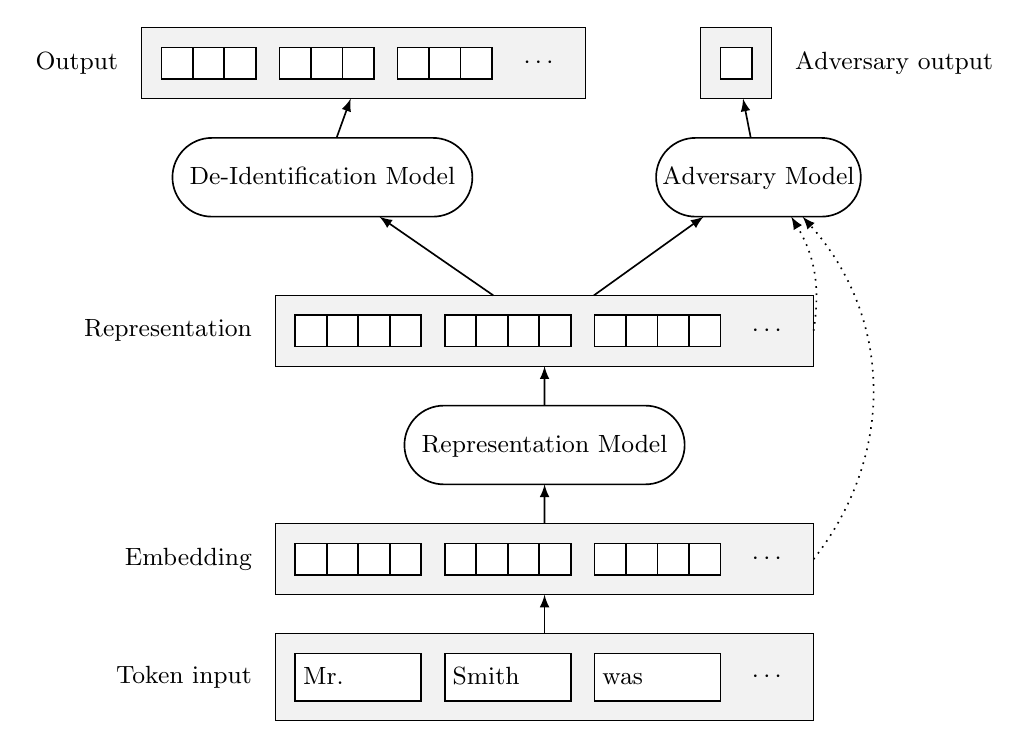
\begin{tikzpicture}[node distance=1.9cm,font=\small]
\tikzset{every node/.style={inner sep=1mm, outer sep=0mm, line width=0mm}}

\tikzstyle{token}=[rectangle,draw=black,fill=white,semithick,text width=1.4cm, minimum width=1.6cm, minimum height=6mm, text height=1.5ex,text depth=.25ex]
\tikzstyle{model}=[rounded rectangle,draw=black,fill=white,semithick, minimum width=3cm, minimum height=10mm, text height=1.5ex,text depth=.25ex, inner sep=2mm]
\tikzstyle{dots} = []
\tikzstyle{vector} = [draw, shape=rectangle, fill=white, semithick, minimum width=1.6cm, minimum height=4mm]
\tikzstyle{half vector} = [shape=rectangle, semithick, minimum width=1.6cm, minimum height=4mm] % without drawn border
\tikzstyle{two thirds vector} = [draw, shape=rectangle, fill=white, semithick, minimum width=1.2cm, minimum height=4mm]
\tikzstyle{quarter vector} = [draw, shape=rectangle, fill=white, semithick, minimum width=4mm, minimum height=4mm]
\tikzstyle{pre}=[<-,semithick, >=latex]
\tikzstyle{post}=[->, semithick, >=latex]

\node[token] (mr input){Mr.};
\node[token, right of=mr input] (smith input) {Smith};
\node[token, right of=smith input] (was input) {was};
\node[dots, right=3mm of was input] (input dots) {$\cdots$};
    
\node[vector, above=10mm of mr input] (mr embedding) {};
\node[vector, right of=mr embedding] (smith embedding) {};
\node[vector, right of=smith embedding] (was embedding) {};
\node[dots, right=3mm of was embedding] (embedding dots) {$\cdots$};

\begin{scope}[on background layer]
    \node (input box) [draw,fill=black!5,fit=(mr input) (input dots), inner sep=2.5mm] {};
    \node (feature box) [draw,fill=black!5,fit=(mr embedding) (embedding dots), inner sep=2.5mm] {};
\end{scope}

\node[model,above=5mm of feature box] (representation model) {Representation Model};

\node[vector, above=2.5cm of mr embedding] (mr representation) {};
\node[vector, right of=mr representation] (smith representation) {};
\node[vector, right of=smith representation] (was representation) {};
\node[dots, right=3mm of was representation] (representation dots) {$\cdots$};

\begin{scope}[on background layer]
    \node (representation box) [draw,fill=black!5,fit=(mr representation) (representation dots), inner sep=2.5mm] {};
\end{scope}

\node[model,above left=1cm and -2cm of representation box] (deid model) {De-Identification Model};

\node[two thirds vector, above left=3cm and 0.5cm of mr representation] (mr output) {};
\node[two thirds vector, right=3mm of mr output] (smith output) {};
\node[two thirds vector, right= 3mm of smith output] (was output) {};
\node[dots, right=3mm of was output] (output dots) {$\cdots$};    

\begin{scope}[on background layer]
 \node (output box) [draw,fill=black!5,fit=(mr output) (output dots), inner sep=2.5mm] {};
\end{scope}

\node[model,above right=1cm and -1.5cm of representation box] (adversary model) {Adversary Model};

\node[quarter vector, above right=3cm and 0cm of was representation] (adversary output) {};

\begin{scope}[on background layer]
    \node (adversary output box) [draw,fill=black!5,fit=(adversary output), inner sep=2.5mm] {};
\end{scope}


% vector squares
\foreach \i in {mr embedding, smith embedding, was embedding, mr representation, smith representation, was representation} {
    \draw[semithick] (\i.north west) rectangle ($(\i.north west) + (4mm, -4mm)$);
    \draw[semithick] (\i.north west) rectangle ($(\i.north west) + (8mm, -4mm)$);
    \draw[semithick] (\i.north west) rectangle ($(\i.north west) + (12mm, -4mm)$);    
};

\foreach \i in {mr output, smith output, was output} {
    \draw[semithick] (\i.north west) rectangle ($(\i.north west) + (4mm, -4mm)$);
    \draw[semithick] (\i.north west) rectangle ($(\i.north west) + (8mm, -4mm)$);
};

\path[post] (input box) edge (feature box);
\path[post] (feature box) edge (representation model);
\path[post] (representation model) edge (representation box);

\path[post] (representation box) edge (deid model);
\path[post] (deid model) edge (output box);

\path[post] (representation box) edge (adversary model);
\path[post,dotted] (feature box.east) edge[bend right=40] (adversary model);
\path[post,dotted] (representation box.east) edge[bend right=20] (adversary model);
\path[post] (adversary model) edge (adversary output box);

\node[anchor=east, left=2mm of input box] {Token input};
\node[anchor=east, left=2mm of feature box] {Embedding};
\node[anchor=east, left=2mm of representation box] {Representation};
\node[anchor=east, left=2mm of output box] {Output};
\node[anchor=west, right=2mm of adversary output box] {Adversary output};

\end{tikzpicture}
        \caption[Adversarial model architecture]{%
            Simplified visualization of the adversarial model architecture.
            %
            Sequences of squares denote real-valued vectors, dotted arrows represent possible additional real or fake inputs to the adversary.
            %
            The casing feature that is provided as a second input to the de-identification model is omitted for legibility.}\label{fig:adversarial-model}
    \end{figure}
    
    \item[Representations]
    %
    We evaluate two types of representation models: a feedforward and \iac{lstm} model.
    %
    Both apply Gaussian noise with zero mean and trainable standard deviations to their inputs and outputs.
    %
    The models learn a standard deviation for each of the input and output dimensions.
    
    %
    We try different representation sizes to explore the trade-off between de-identification and adversary performances.
    %
    In contrast to the approaches from \cref{sec:perturbing} that only perturb \ac{phi} tokens, the representation models in this approach process all tokens to represent them in a new embedding space.
    
    \item[Adversaries]
    %
    In existing gradient reversal approaches \citep{ganin2016domain,feutry2018learning,elazar2018adversarial}, the learned representation is invariant to some attribute of the input.
    %
    Similarly, our representation should be invariant to small input changes, like a single token being replaced with a neighbor in the embedding space.
    %
    The number of neighbors $N$ controls the privacy properties of the representation.
    
    %
    Additionally, we need our representation to contain a random element because we want to share the output representations as well as the representation model itself.
    %
    An attacker should not be able to create a lookup table of representations for exact sentences, i.e.\ the representation must be immune to known-plaintext attacks.
    
    %
    To achieve these goals, we use two adversaries that are trained for the following tasks:
    \begin{enumerate}
        \item Given a representation and an embedding sequence, decide if they were obtained from the same sentence.
        \item Given two representation sequences (and their cosine similarities), decide if they were obtained from the same sentence.
    \end{enumerate}
    
    %
    \Cref{fig:adversaries} shows the two adversaries with their respective inputs.
    %
    The first adversary's objective is a discriminatory formulation of an inverse representation model and causes representations for similar inputs (replacing any protected token with one of its $N$ neighbors) to be indistinguishable.
    %
    The second adversary's objective causes repeated representation computations for the same sentence to differ by a high enough degree to make it impossible to build a lookup table of representations.
    %
    We obtain the representation sequences for the second adversary from copies of the representation model with shared weights.
    %
    We generate real and fake pairs for adversarial training using the automatic pseudonymization approach presented in \cref{sec:auto-pseudo}, limiting the number of replaced tokens to one per sentence.
    
    %
    The adversaries are implemented as bidirectional \ac{lstm} models.
    %
    We confirmed that bidirectional \ac{lstm} models are able to learn the adversarial tasks on randomly generated data and raw word embeddings in a preliminary experiment.
    %
    To use the two adversaries in our architecture, we average their outputs.
    
    \item[Training]
    %
    We evaluate two training procedures: \ac{dann} training~\citep{ganin2016domain} and the alternating approach by \citet{feutry2018learning}.
    
    %
    In \ac{dann} training, the three components are trained conjointly, optimizing the sum of losses.
    %
    Training the de-identification model modifies the representation model weights to generate a more meaningful representation for de-identification.
    %
    The adversary gradient is reversed with a gradient reversal layer between the adversary and the representation model in the backward pass, causing the representation to become less meaningful for the adversary.
    
    %
    The training procedure by \citet{feutry2018learning} is shown in \cref{fig:feutry-training}.
    %
    It is composed of three sequential phases:
    %
    \begin{enumerate}
        \item The de-identification and representation models are pre-trained together, optimizing the de-identification loss $L_{\text{deid}}$.
        \item The representation model is frozen and the adversary is pre-trained, optimizing the adversarial loss $L_{\text{adv}}$.
        \item In alternation, for one epoch each:
        \begin{enumerate}
            \item The representation is frozen and both de-identification model and adversary are trained, optimizing their respective losses $L_{\text{deid}}$ and $L_{\text{adv}}$.
            \item The de-identification model and adversary are frozen and the representation is trained, optimizing the combined loss $L_{\text{repr}} = L_{\text{deid}} + \lambda \abs{L_{\text{adv}} - L_{\text{random}}}$. \label{item:repr-training}
        \end{enumerate}
    \end{enumerate}
    
    \begin{figure}
        \centering
        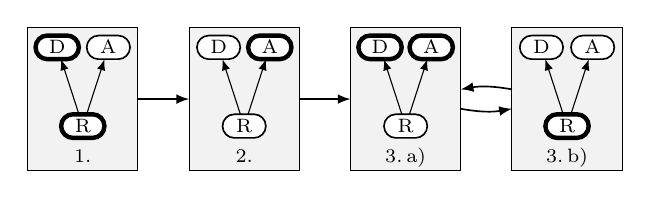
\begin{tikzpicture}[node distance=1.5cm,font=\scriptsize, sibling distance=6.5mm, level distance=1cm, grow=up, edge from parent/.style = {->, >=latex, draw}]
\tikzset{every node/.style={inner sep=0mm, outer sep=0mm, line width=0mm}}

\tikzstyle{model}=[rounded rectangle,draw=black,fill=white, minimum width=5.5mm, minimum height=3mm, semithick, text depth=-.2ex]
\tikzstyle{train}=[ultra thick]
\tikzstyle{label}=[text height=0.75ex,text depth=0ex]
\tikzstyle{dots} = []
\tikzstyle{pre}=[<-,semithick, >=latex]
\tikzstyle{post}=[->, semithick, >=latex]

\node[model, train] (a) {R}
    child {node[model] (a adv) {A}}
    child {node[model, train] (a deid) {D}};

\node[label, below= 2mm of a] (a label) {1.}; 

\node[model, right=of a] (b) {R}
    child {node[model, train] (b adv) {A}}
    child {node[model] (b deid) {D}};

\node[label, below=2mm of b] (b label) {2.}; 

\node[model, right=of b] (c) {R}
    child {node[model, train] (c adv) {A}}
    child {node[model, train] (c deid) {D}};
    
\node[label, below=2mm of c] (c label) {3.$\,$a)}; 

\node[model, right= of c, train] (d) {R}
    child {node[model] (d adv) {A}}
    child {node[model] (d deid) {D}};
    
\node[label, below=2mm of d] (d label) {3.$\,$b)}; 
    
\begin{scope}[on background layer]
    \node (a box) [draw,fill=black!5,fit=(a) (a label) (a adv) (a deid), inner sep=1mm] {};
    \node (b box) [draw,fill=black!5,fit=(b) (b label) (b adv) (b deid), inner sep=1mm] {};
    \node (c box) [draw,fill=black!5,fit=(c) (c label) (c adv) (c deid), inner sep=1mm] {};
    \node (d box) [draw,fill=black!5,fit=(d) (d label) (d adv) (d deid), inner sep=1mm] {};
\end{scope}

\path[post] (a box) edge (b box);
\path[post] (b box) edge (c box);
\path[post] (c box) edge[bend right=10] (d box);
\path[post] (d box) edge[bend right=10] (c box);

\end{tikzpicture}
        \caption[Adversarial training procedure]{%
            Visualization of \citeauthor{feutry2018learning}'s training procedure.
            %
            The adversarial model layout follows \cref{fig:adversarial-model}: the representation model is at the bottom, the left branch is the de-identification model and the right branch is the adversary.
            %
            In each step, the thick components are trained while the thin components are frozen.
            %
            Steps 1 and 2 are trained until stable.
            %
            Then training alternates between one epoch and step 3a and one epoch of step 3b.
        }\label{fig:feutry-training}
    \end{figure}
    
    %
    In the first two phases, we monitor the respective validation losses for early stopping to decide at which point the training should move on to the next phase.
    %
    The alternating steps in the third phase each last one training epoch.
    %
    We determine the early stopping epoch using only the combined validation loss (\cref{item:repr-training}).
    
    %
    Gradient reversal is achieved by optimizing the combined representation loss while the adversary weights are frozen.
    %
    The combined loss is motivated by the fact that the adversary performance should be the same as a random guessing model, which is a lower bound for anonymization~\citep{feutry2018learning}.
    %
    The term $\abs{L_{\text{adv}} - L_{\text{random}}}$ approaches $0$ when the adversary performance approaches random guessing\footnote{In the case of binary classification: $L_{\text{random}} = -\log \frac{1}{2} \approx 0.6931$.}.
    %
    $\lambda$ is a weighting factor for the two losses; we select $\lambda=1$.
    
    \item[Application]
    %
    To apply the model in practice, a central model provider would train the three parts of the model on an initial \ac{phi}-annotated dataset, e.g.\ the i2b2 2014 data.
    %
    This initial training should confirm that the learned representation allows training a de-identification model while being robust to the adversaries.
    %
    The model provider would then publish the representation model along with their choice of pre-trained word embeddings.
    %
    Medical institutions would use the representation model to transform their \ac{phi}-labeled data into a private representation, which is then sent back to the central model provider with the respective labels.
    %
    This transformation replaces the manual document-coherent pseudonymization that is typically performed to share training data for de-identification.
    
    %
    The model provider would then update the existing de-identification model or train a new model using all available representation data.
    %
    Periodically, the pipeline of representation model (possibly in a version without additive noise) and de-identification model would be published so it can be used by medical institutions on their unlabeled data.
\end{description}
% !TeX root=main
% !TeX spellcheck=en_US

\section{Discussion}\label{sec:discussion}

\subsection{De-Identification Performance}

\subsection{Privacy Properties}


% !TeX root=main
% !TeX spellcheck=en_US

\section{Conclusions}\label{sec:conclusions}

%\section*{Acknowledgments}
%Deidentified clinical records used in this research were provided by the i2b2 National Center for Biomedical Computing funded by U54LM008748 and were originally prepared for the Shared Tasks for Challenges in NLP for Clinical Data organized by Dr.\ Özlem Uzuner, i2b2 and SUNY.

% include your own bib file like this:
%\bibliographystyle{acl}
%\bibliography{acl2018}
\bibliography{deidentification-clean}
\bibliographystyle{acl_natbib}

\end{document}
